\ifx\wholebook\relax \else
\documentclass[b5paper]{article}
\usepackage[nomarginpar
  %, margin=.5in
]{geometry}

\addtolength{\oddsidemargin}{-0.05in}
\addtolength{\evensidemargin}{-0.05in}
\addtolength{\textwidth}{0.1in}
\usepackage[en]{../../../prelude}

\setcounter{page}{1}

\begin{document}

\title{Sequence}

\author{Xinyu~LIU
\thanks{{\bfseries Xinyu LIU} \newline
  Email: liuxinyu95@gmail.com \newline}
  }

\maketitle
\fi

\markboth{Sequence}{Elementary Algorithms}

\ifx\wholebook\relax
\chapter{Sequence}
\numberwithin{Exercise}{chapter}
\fi

\section{Introduction}
\label{introduction}

Sequence is the combination of array and list. We set the following goals for the ideal sequence:

\begin{enumerate}
\item Add, remove element on head and tail in constant time;
\item Fast (no slower than linear time) concatenate two sequences;
\item Fast access, update element at any position;
\item Fast split at any position;
\end{enumerate}

Array and list only satisfy these goals partially as shown in below table, where $n$ is the length for the sequence, and use $n_1$, $n_2$ for lengths if there are two.

\btab{| l | l | l |}
  \hline
  operation & array & list \\
  \hline
  add/remove on head & $O(n)$ & $O(1)$ \\
  add/remove on tail & $O(1)$ & $O(n)$ \\
  concatenate & $O(n_2)$ & $O(n_1)$ \\
  random access at $i$ & $O(1)$ & $O(i)$ \\
  remove at $i$ & $O(n-i)$ & $O(i)$ \\
  \hline
\etab

We give three implementations: binary random access list, concatenate-able list, and finger tree.

\section{Binary random access list}
\index{Sequence!Binary random access list}

The binary random access list is a set of full binary trees (forest). The elements are stored in leaves. For any integer $n \geq 0$, we know how many trees need to hold $n$ elements from its binary format. Every bit of 1 represents a binary tree, the tree size is determined by the magnitude of the bit. For any index $1 \leq i \leq n$, we can locate the binary tree that stores the $i$-th element. As shown in \cref{fig:bi-tree-sequence}, tree $t_1, t_2$ represent sequence $[x_1, x_2, x_3, x_4, x_5, x_6]$.

\begin{figure}[htbp]
  \centering
  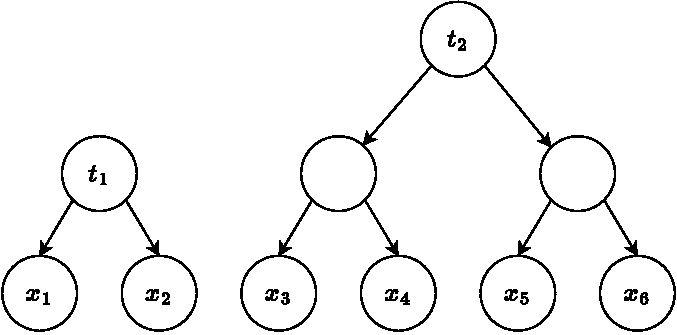
\includegraphics[scale=0.6]{img/bi-tree-sequence}
  \caption{A sequence of 6 elements.}
  \label{fig:bi-tree-sequence}
\end{figure}

Denote the full binary tree of depth $i + 1$ as $t_i$. $t_0$ only has a leaf node. There are $2^i$ leaves in $t_i$. For sequence of $n$ elements, represent $n$ in binary as $n = (e_m e_{m-1} ... e_1 e_0)_2$, where $e_i$ is either 1 or 0.

\be
n = 2^0 e_0 + 2^1 e_1 + ... + 2^m e_m
\ee

If $e_i \neq 0$, there is a full binary tree $t_i$ of size $2^i$. For example in \cref{fig:bi-tree-sequence}, the length of the sequence is $6 = (110)_2$. The lowest bit is 0, there's no tree of size 1; the 2nd bit is 1, there is $t_1$ of size 2; the highest bit is 1, there is $t_2$ of size 4. In this way, we represent sequence $[x_1, x_2, ..., x_n]$ as a list of trees. Each tree has unique size, in ascending order. We call it {\em binary random access list}\cite{okasaki-book}. Customize the binary tree definition: (1) only store the element in leaf node as $(x)$; (2) augment the size in each branch node as $(s, l, r)$, where $s$ is the size of the tree, $l$, $r$ are left and right sub-trees respectively. We get the size as below:

\be
\begin{array}{rcl}
size\ (x) & = & 1 \\
size\ (s, l, r) & = & s \\
\end{array}
\ee

\index{Binary Random Access List!insert}
To add a new element $y$ before sequence $S$, we create a singleton $t_0$ tree $t' = (y)$, then insert it to the forest. $insert\ y\ S = insert_T\ (y)\ S$, or in Curried form:

\be
insert\ y = insert_T\ (y)
\ee

Compare $t'$ with the first tree $t_i$ in the forest, if $t_i$ is bigger, then put $t'$ ahead of the forest (in constant time); if they have the same size, then link them to a bigger tree (in constant time): $t'_{i+1} = (2s, t_i, t')$, then recursively insert $t'_{i+1}$ to the forest, as shown in \cref{fig:bralist-2}.

\be
\begin{array}{rcl}
insert_T\ t\ [\ ] & = & [t] \\
insert_T\ t\ (t_1 \cons ts) & = & \begin{cases}
  size\ t < size\ t_1: & t : t_1 : ts \\
  \text{otherwise}: & insert_T\ (link\ t\ t_1)\ ts \\
  \end{cases}
\end{array}
\ee

Where: $link\ t_1\ t_2 = (size\ t_1 + size\ t_2, t_1, t_2)$.

\begin{figure}[htbp]
  \centering
  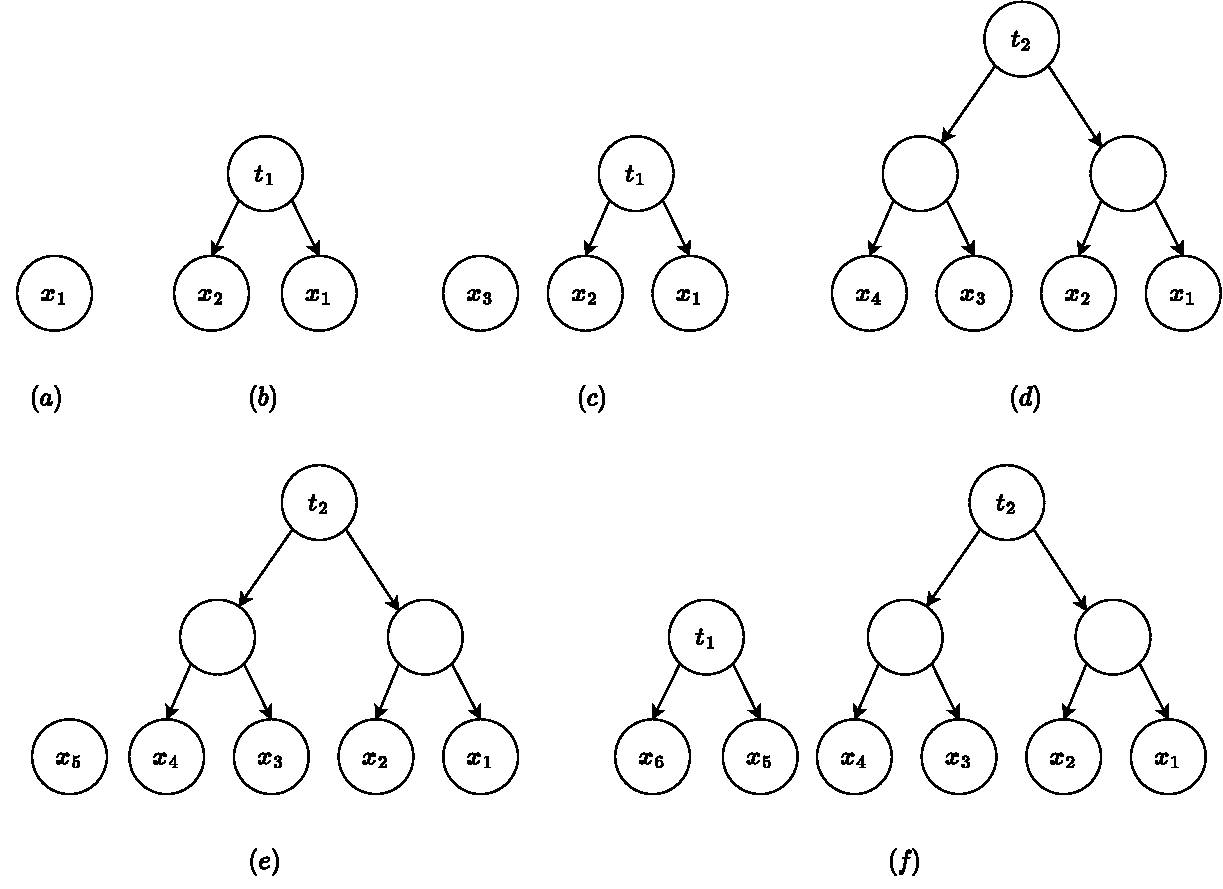
\includegraphics[scale=0.55]{img/bralst-add}
  \caption{Insert $x_1, x_2, ..., x_6$. (a) Insert $x_1$, (b) Insert $x_2$, link to $[t_1]$. (c) Insert $x_3$, result $[t_0, t_1]$. (d) Insert $x_4$, link twice, generate $[t_2]$. (e) Insert $x_5$, result $[t_0, t_2]$. (f) Insert $x_6$, result $[t_1, t_2]$.}
  \label{fig:bralist-2}
\end{figure}

For $n$ elements, there are $m = O(\lg n)$ trees in the forest. The performance is bound to $O(\lg n)$ time. We'll prove the amortized performance is constant time.

\index{Binary Random Access List!remove}

We define remove conversely. If the first tree is $t_0$ (singleton leaf), then remove it; otherwise, recursively split the first tree to obtain a $t_0$ and remove, as shown in \cref{fig:bralist-pop}.

\begin{figure}[htbp]
  \centering
  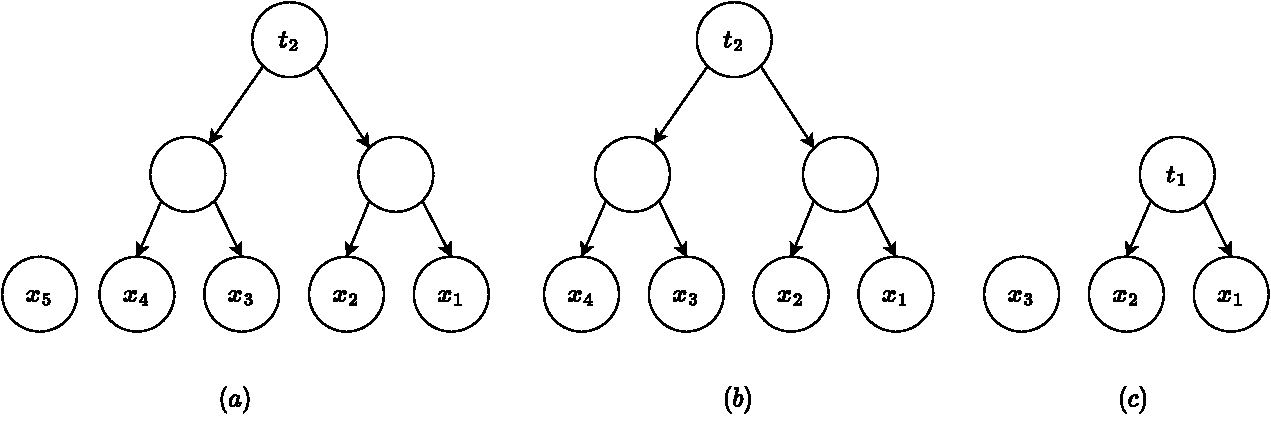
\includegraphics[scale=0.55]{img/bralst-remove}
  \caption{Remove: (a) $x_1, x_2, ..., x_5$ as $[t_0, t_2]$. (b) Remove $x_5$ ($t_0$) directly. (c) Remove $x_4$. Split twice to get $[t_0, t_0, t_1]$, then remove the head to get $[t_0, t_1]$.}
  \label{fig:bralist-pop}
\end{figure}

\be
\begin{array}{rcl}
extract\ ((x) \cons ts) & = & (x, ts) \\
extract\ ((s, t_1, t_2) \cons ts) & = & extract\ (t_1 \cons t_2 \cons ts) \\
\end{array}
\ee

We call $extract$ to remove element from head:

\be
\begin{cases}
head & = \textit{fst} \circ extract \\
tail & = \textit{snd} \circ extract \\
\end{cases}
\ee

Where $\textit{fst}\ (a, b) = a$, $\textit{snd}\ (a, b) = b$ access the component in a pair.

\index{Binary Random Access List!random access}

The trees divide elements into chunks. For a given index $1 \leq i \leq n$, first locate the corresponding tree, then lookup the tree to access the element.

\begin{enumerate}
\item For the first tree $t$ in the forest, if $i \leq size(t)$, then the element is in $t$, we next lookup $t$ for the target element;
\item Otherwise, let $i' = i - size(t)$, then recursively lookup the $i'$-th element in the rest trees.
\end{enumerate}

\be
(t \cons ts)[i] = \begin{cases}
  i \leq size\ t: & lookup_T\ i\ t \\
  \text{otherwise}: & ts[i - size\ t] \\
\end{cases}
\ee

Where $lookup_T$ applies binary search. If $i = 1$, returns the root, else divides the tree and recursively looks up:

\be
\begin{array}{rcl}
lookup_T\ 1\ (x) & = & x \\
lookup_T\ i\ (s, t_1, t_2) & = & \begin{cases}
  i \leq \lfloor \dfrac{s}{2} \rfloor: & lookup_T\ i\ t_1 \\
  \text{otherwise}: & lookup_T\ (i - \lfloor \dfrac{s}{2} \rfloor)\ t_2 \\
  \end{cases}
\end{array}
\ee

\Cref{fig:get-at-example} gives the steps to lookup the 4-th element in a sequence of length 6. The size of the first tree is 2 < 4, move to the next tree and update the index to $i' = 4 - 2$. The size of the second tree is $4 > i' = 2$, we need lookup it. Because the index 2 is less than the half size $4/2 = 2$, we lookup the left, then the right, and finally locate the element. Similarly, we can alter an element at a given position.

\begin{figure}[htbp]
  \centering
  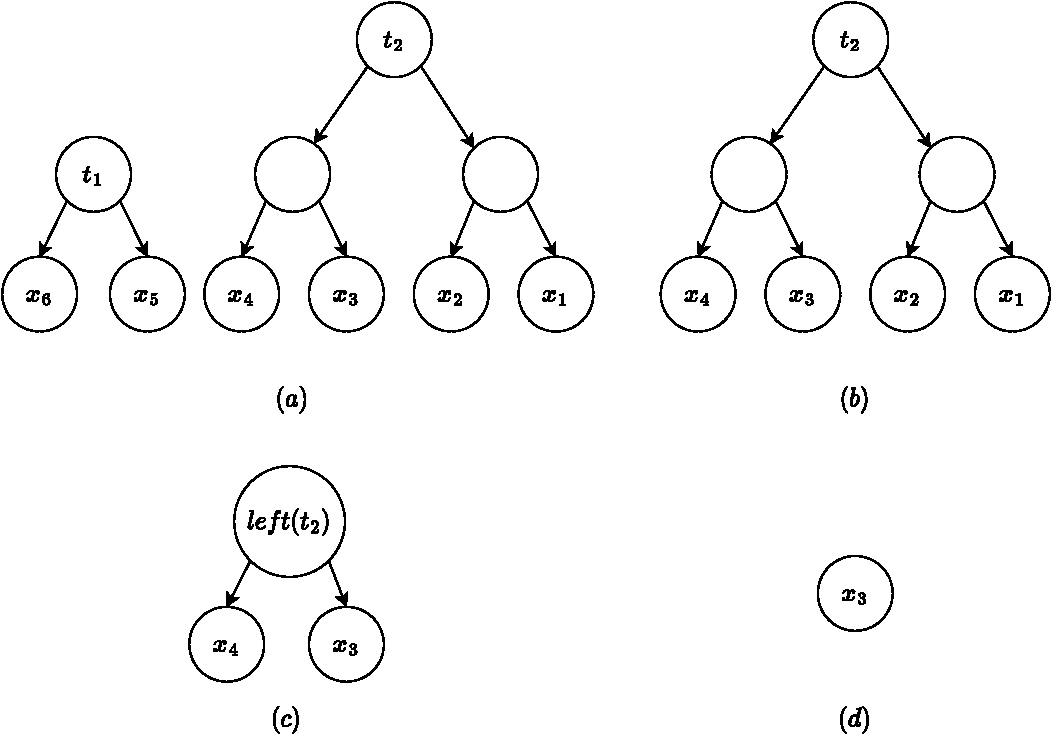
\includegraphics[scale=0.55]{img/bralst-index}
  \caption{Steps to access $S[4]$: (a) $S[4], 4 > size(t_1) = 2$, (b) $S'[4-2] \Rightarrow lookup_T\ 2\ t_2$, (c) $ 2 \leq \lfloor \dfrac{size(t_2)}{2} \rfloor \Rightarrow lookup_T\ 2\ left(t_2)$, (d) $lookup_T\ 1\ right(left(t_2))$, return $x_3$.}
  \label{fig:get-at-example}
\end{figure}

There are $O(\lg n)$ full binary trees to hold $n$ elements. For index $i$, we need at most $O(\lg n)$ time to locate the tree, the next lookup time is proportion to the height, which is $O(\lg n)$ at most. The overall random access time is bound to $O(\lg n)$.

\begin{Exercise}\label{ex:bralist-idx-bound}
How to handle the out of bound exception?
\end{Exercise}

\begin{Answer}[ref = {ex:bralist-idx-bound}]
How to handle the out of bound exception?

We can use Mybe type to handle the out of bound cases. If the index $i < 0$, return Nothing, if the index exceeds, then it eventually converts to empty forest after recursion, we return Nothing in this case too.

\begin{Haskell}
getAt [] _ = Nothing
getAt (t:ts) i | i < 0 = Nothing
               | i < size t = lookupTree i t
               | otherwise = getAt ts (i - size t)
  where
    lookupTree 0 (Leaf x) = Just x
    lookupTree i (Node sz t1 t2) | i < sz `div` 2 = lookupTree i t1
                                 | otherwise = lookupTree (i - sz `div` 2) t2
\end{Haskell}
\end{Answer}

\section{Numeric representation}
\index{Sequence!numeric representation}

The binary form of $n = 2^0e_0 + 2^1e_1 + ... + 2^me_m$ maps to the forest. The $e_i$ is the $i$-th bit. If $e_i = 1$, there is a full binary tree of size $2^i$. Adding an element corresponds to +1 to a binary number; while deleting corresponds to -1. We call such correspondence {\em numeric representation}\cite{okasaki-book}. To explicitly express this correspondence, we define two states: $Zero$ means none existence of the binary tree, while $One\ t$ means there exits tree $t$. As such, we represent the forest as a list of binary states, and implement insert as binary add.

\be
\begin{array}{rcl}
add\ t\ [\ ] & = & [One\ t] \\
add\ t\ (Zero \cons ds) & = & (One\ t) : ds \\
add\ t\ (One\ t' \cons ds) & = & Zero : add\ (link\ t\ t')\ ds
\end{array}
\ee

When add tree $t$, if the forest is empty, we create a state of $One\ t$, it's the only bit, corresponding to $0 + 1 = 1$. If the forest isn't empty, and the first bit is $Zero$, we use the state $One\ t$ to replace $Zero$, corresponding to binary add $(...digits...0)_2 + 1 = (...digits...1)_2$. For e.g. $6 + 1 = (110)_2 + 1 = (111)_2 = 7$. If the first bit is $One\ t'$, we assume $t$ and $t'$ have the same size because we always start to insert from a singleton leaf $t_0 = (x)$. The tree size increase as a sequence of $1, 2, 4, ..., 2^i, ...$. We link $t$ and $t'$, recursively insert to the rest bits. The original $One\ t'$ is replaced by $Zero$. It corresponds to binary add $(...digits...1)_2 + 1 = (...digits'...0)_2$. For e.g. $7 + 1 = (111)_2 + 1 = (1000)_2 = 8$.

Symmetrically, we implement remove as binary subtraction. If the sequence is a singleton bit $One\ t$, it becomes empty after remove, corresponding to $1 - 1 = 0$. If there are multiple bits and the first one is $One\ t$, we replace it by $Zero$. This corresponds to $(...digits...1)_2 - 1 = (...digits...0)_2$. For e.g., $7 - 1 = (111)_2 - 1 = (110)_2 = 6$. If the first bit is $Zero$, we need borrow. We cursively extract tree from the rest bits, split into two $t_1, t_2$, replace $Zero$ to $One\ t_2$, and remove $t_1$. It corresponds to $(...digits...0)_2 - 1 = (...digits'...1)_2$. For e.g., $4 - 1 = (100)_2 - 1 = (11)_2 = 3$.

\be
\begin{array}{rcl}
minus\ [One\ t] & = & (t, [\ ]) \\
minus\ ((One\ t) \cons ts) & = & (t, Zero \cons ts) \\
minus\ (Zero \cons ts) & = & (t_1, (One\ t_2) \cons ts'), \text{where}: (s, t_1, t_2) = minus\ ts \\
\end{array}
\ee

Numeric representation doesn't change the performance. We next evaluate the amortized time by aggregation. The steps to insert $n = 2^m$ elements to empty is given as \cref{tab:ralist-insertion}:

\begin{table}[htbp]
\centering
\begin{tabular}{| l | r |}
  \hline
  i & binary (MSB ... LSB) \\
  \hline
  0 & 0, 0, ..., 0, 0 \\
  1 & 0, 0, ..., 0, 1 \\
  2 & 0, 0, ..., 1, 0 \\
  3 & 0, 0, ..., 1, 1 \\
  ... & ... \\
  $2^m-1$ & 1, 1, ..., 1, 1 \\
  $2^m$ & 1, 0, 0, ..., 0, 0 \\
  \hline
  bits changed & 1, 1, 2, ... $2^{m-1}$, $2^m$ \\
  \hline
\end{tabular}
\caption{Insert $2^m$ elements.}
\label{tab:ralist-insertion}
\end{table}

The LSB changes every time when insert, total $2^m$ times. The second bit changes every other time (link trees), total $2^{m - 1}$ times. The second highest bit only changes 1 time, links all trees to the final one. The highest bit changes to 1 after insert the last element. Sum as: $T = 1 + 1 + 2 + 4 + ... + 2^{m-1} + 2^m = 2^{m+1}$. Hence the amortized performance is:

\be
O(T/n) = O(\dfrac{2^{m+1}}{2^m}) = O(1)
\ee

Proved the amortized constant time performance.

\begin{Exercise}\label{ex:num-representaion}
\Question{Implement the random access for numeric representation $S[i], 1 \leq i \leq n$, where $n$ is the length of the sequence.}
\Question{Analyze the amortized performance of delete.}
\Question{We can represent the full binary tree with array of length $2^m$, where $m$ is none negative integer. Implement the binary tree forest, insert, and random access.}
\end{Exercise}

\begin{Answer}[ref = {ex:num-representaion}]
\Question{Implement the random access for numeric representation $S[i], 1 \leq i \leq n$, where $n$ is the length of the sequence.

We skip the index out of bound exception:
\begin{Haskell}
getAt (Zero:ts) i = getAt ts i
getAt (One t:ts) i = if i < size t then lookupTree t i
                     else getAt ts (i - size t)
  where
    lookupTree (Leaf x) 0 = x
    lookupTree (Node sz t1 t2) i = if i < sz `div` 2 then lookupTree t1 i
                                   else lookupTree t2 (i - sz `div` 2)
\end{Haskell}
}
\Question{Analyze the amortized performance of delete.

Consider the reverse process of insert, delete from a sequence with $n = 2^m$ elements repeatedly till it becomes empty. The analysis is symmetric to insert, and it gives the amortized constant time.
} %amortized O(1)
\Question{We can represent the full binary tree with array of length $2^m$, where $m$ is none negative integer. Implement the binary tree forest, insert, and random access.

\begin{Bourbaki}
data List<K> {
    Int size = 0
    [[K]] trees = [[]]
}

Int nbits(Int n) {
    Int i = 0
    while n != 0 {
        i = i + 1
        n = n / 2
    }
    return i
}

List<K> insert(List<K> xs, K x) {
    var i = nbits(xs.size xor (1 + xs.size))    // locate the bit flip to 1
    if i >= length(xs.trees) then xs.trees.append([])
    xs.trees[i] = [x]
    for Int j = 0, j < i, j++ {
        xs.trees[i] = xs.trees[i] ++ xs.trees[j]
        xs.trees[j] = []
    }
    xs.size = xs.size + 1
    return xs
}

Optional<K> get(List<K> xs, Int i) {
    for t in xs.trees {
        Int size = length(t)
        if i < size then return Optional.of(t[i])
        i = i - size
    }
    return Optional.Nothing
}
\end{Bourbaki}
}
\end{Answer}

\section{paired-array sequence}
\index{Sequence!Paired-array sequence}

Expand the paired-array queue (see chapter 11) to paired-array sequence. As shown in \cref{fig:parrays}, link two arrays head to head. When add an element from left, we append to the tail of $f$; when add from right, we append to the tail of $r$. Denote the sequence as a pair $S = (f, r)$, $\textproc{Front}(S) = f$, $\textproc{Rear}(S) = r$ access them respectively. Implement insert/append as below:

\begin{figure}[htbp]
  \centering
  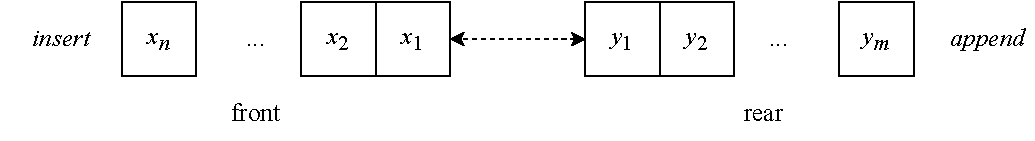
\includegraphics[scale=0.7]{img/parrays}
  \caption{Paired-array sequence.}
  \label{fig:parrays}
\end{figure}

\begin{algorithmic}[1]
\Function{Insert}{$x, S$}
  \State \textproc{Append}($x$, \Call{Front}{$S$})
\EndFunction
%\Statex
\Function{Append}{$x, S$}
  \State \textproc{Append}($x$, \Call{Rear}{$S$})
\EndFunction
\end{algorithmic}

\index{Paired-array sequence!random access}

When access the $i$-th element, we first determine which array $i$ indexes to, $f$ or $r$? If $ i \leq |f|$, the element is in $f$. Because $f$ and $r$ are connected head to head, we need index from right of $f$ at position $|f| - i + 1$; if $i > |f|$, the element is in $r$. We index from left at position $i - |f|$.

\begin{algorithmic}[1]
\Function{Get}{$i, S$}
  \State $f, r \gets $ \Call{Front}{$S$}, \Call{Rear}{$S$}
  \State $n \gets $ \Call{Size}{$f$}
  \If{$i \leq n $}
    \State \Return $f[n - i + 1]$ \Comment{reversed}
  \Else
    \State \Return $r[i - n]$
  \EndIf
\EndFunction
\end{algorithmic}

\index{Paired-array sequence!remove and balance}
Removing can make $f$ or $r$ empty ($[\ ]$), while the other is not. To re-balance, we halve the none empty one, and reverse either half to form a new pair. As $f$ and $r$ are symmetric, we can swap them, call \textproc{Balance}, then swap back.

\begin{algorithmic}[1]
\Function{Balance}{$S$}
  \State $f \gets$ \Call{Front}{$S$}, $r \gets$ \Call{Rear}{$S$}
  \State $n \gets$ \Call{Size}{$f$}, $m \gets$ \Call{Size}{$r$}
  \If{$F = [\ ]$}
    \State $k \gets \lfloor \dfrac{m}{2} \rfloor$
    \State \Return $(\textproc{Reverse}(r[1 ... k]), r[(k + 1) ... m])$
  \EndIf
  \If{$R = [\ ]$}
    \State $k \gets \lfloor \dfrac{n}{2} \rfloor$
    \State \Return $(f[(k + 1) ... n], \textproc{Reverse}(f[1 ... k]))$
  \EndIf
  \State \Return $(f, r)$
\EndFunction
\end{algorithmic}

Every time when delete, we check $f$, $r$ and balance them:

\begin{algorithmic}[1]
\Function{Remove-Head}{$S$}
  \State \Call{Balance}{$S$}
  \State $f, r \gets$ \Call{Front}{$S$}, \Call{Rear}{$S$}
  \If{$f = [\ ]$} \Comment{$S = ([], [x])$}
    \State $r \gets [\ ]$
  \Else
    \State \Call{Remove-Last}{$f$}
  \EndIf
\EndFunction
\Statex
\Function{Remove-Tail}{$S$}
  \State \Call{Balance}{$S$}
  \State $f, r \gets$ \Call{Front}{$S$}, \Call{Rear}{$S$}
  \If{$r = [\ ]$} \Comment{$S = ([x], [])$}
    \State $f \gets [\ ]$
  \Else
    \State \Call{Remove-Last}{$r$}
  \EndIf
\EndFunction
\end{algorithmic}

Due to reverse, the performance is $O(n)$ in the worst case, where $n$ is the number of elements, while it is amortized constant time.

\begin{Exercise}\label{ex:paired-array-seq}
Analyze the amortized performance for paired-array delete.
\end{Exercise}

\begin{Answer}[ref = {ex:paired-array-seq}]
Analyze the amortized performance for paired-array delete.

Define the potential of the paired-array sequence as the difference of the array lengths: $\Phi(s) = |r| - |f| = n - m$, where $m = |f|$ and $n = |r|$. When delete from the head, if $f \neq []$, then takes $O(1)$ time to remove the last element of $f$. If $f = []$, the takes $O(n)$ time to halve $r$, reverse and replace as $f'$. Then use another $O(1)$ time to remove the last element of $f'$. The amortized cost is:

\[
\begin{array}{rcl}
c & = & n + 1 + \Phi(s') - \Phi(s) \\
  & = & n + 1 + (|r'| - |f'|) - (|r| - |f|) \\
  & = & n + 1 + (n - \lceil \dfrac{n}{2} \rceil) - (\lceil \dfrac{n}{2} \rceil - 1) -  (n - 0) \\
  & = & 1 \\
\end{array}
\]

Hence the amortized time is $O(1)$ when delete from head, symmetrically, the amortized time is $O(1)$ when delete from tail too.
\end{Answer}

\section{Concatenate-able list}
\index{Sequence!Concatenate-able list}

We achieve $O(\lg n)$ time insert, delete, random index with binary tree forest. However, it's not easy to concatenate two sequences. We can't merely merge trees, but need link trees with the same size. \Cref{fig:clist} shows an implementation of concatenate-able list. The first element $x_1$ is in root, the rest is organized with smaller sequences, each one is a sub-tree. These sub-trees are put in a real-time queue (see chapter 11). We denote the sequence as $(x_1, Q_x) = [x_1, x_2, ..., x_n]$. When concatenate with another sequence of $(y_1, Q_y) = [y_1, y_2, ..., y_m]$, we append it to $Q_x$. The real-time queue guarantees the en-queue in constant time, hence the concatenate performance is in constant time.

\begin{figure}[htbp]
  \centering
  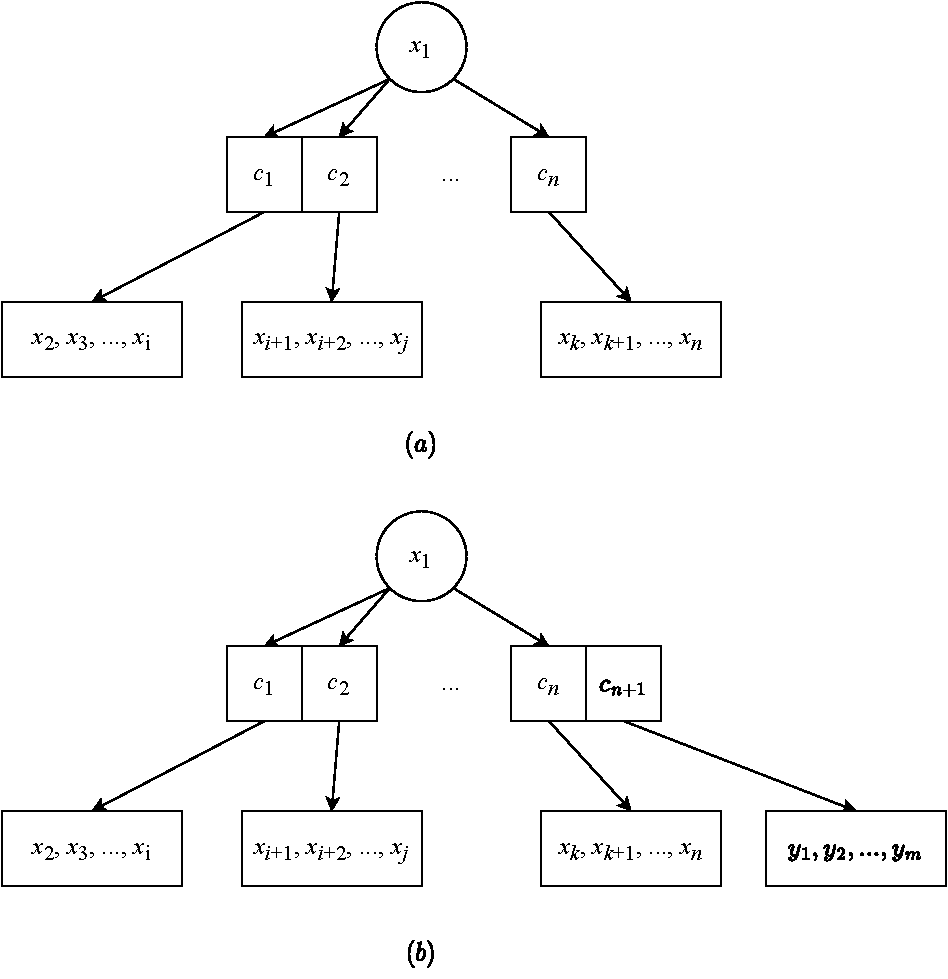
\includegraphics[scale=0.6]{img/clist}
  \caption{Concatenate-able list: (a) $(x_1, Q_x) = [x_1, x_2, ..., x_n]$, (b) Concatenate with $(y_1, Q_y) = [y_1, y_2, ..., y_m]$, add$c_{n+1}$ to $Q_x$.}
  \label{fig:clist}
\end{figure}

\be
\begin{array}{rcl}
s \doubleplus \nil & = & s \\
\nil \doubleplus s & = & s \\
(x, Q) \doubleplus s & = & (x,\ push\ s\ Q) \\
\end{array}
\ee

When insert new element $z$, we create a singleton of $(z, \nil)$, then concatenate it to the sequence:

\be
\begin{cases}
insert\ x\ s & = (x, \nil) \doubleplus s \\
append\ x\ s & = s \doubleplus (x, \nil) \\
\end{cases}
\ee

When delete $x_1$ from head, we lose the root. The rest sub-trees are all concatenate-able lists. We concatenate them together to a new sequence.

\be
\begin{array}{rcl}
concat\ \nil & = & \nil \\
concat\ Q & = & (top\ Q) \doubleplus concat\ (pop\ Q) \\
\end{array}
\ee

The real-time queue holds sub-trees, we pop the first $c_1$, and recursively concatenate the rest to $s$, then concatenate $c_1$ and $s$. We define delete from head with $concat$.

\be
tail\ (x, Q) = concat\ Q
\ee

Function $concat$ traverses the queue, and reduces to a result, it essentially folds on $Q$\cite{learn-haskell}.

\be
\begin{array}{rcl}
fold\ f\ z\ \nil & = & z \\
fold\ f\ z\ Q & = & f\ (top\ Q)\ (fold\ f\ z\ (pop\ Q)) \\
\end{array}
\ee

Where $f$ is a binary function, $z$ is zero unit. Here are examples of folding on queue $Q = \{1, 2, ..., 5\}$:

\[
\begin{array}{rcl}
fold\ (+)\ 0\ Q & = & 1 + (2 + (3 + (4 + (5 + 0)))) = 15 \\
fold\ (\times)\ 1\ Q\ & = & 1 \times (2 \times (3 \times (4 \times (5 \times 1)))) = 120 \\
fold\ (\times)\ 0\ Q & = & 1 \times (2 \times (3 \times (4 \times (5 \times 0)))) = 0 \\
\end{array}
\]

We can define $concat$ with fold (Curried form):

\be
concat = fold\ (\doubleplus)\ \nil
\ee

Normally, the add, append, delete randomly happen. The performance is bound to linear time in worst case: delete after repeatedly add $n$ elements. All $n-1$ sub-trees are singleton. $concat$ takes $O(n)$ time to consolidate. Nevertheless, the amortized performance is constant time.

%% \begin{Exercise}
%% \Question{Prove the amortized performance for delete is constant time} %Banker method.
%% \end{Exercise}

\section{Finger tree}
\index{Sequence!finger tree}

Binary random access list supports to insert, remove from head in amortized constant time, and index in logarithm time. But we can't easily append element to tail, or fast concatenate. With concatenate-able list, we can concatenate, insert, and append in amortized constant time, but can't easily index element. From these two examples, we need: (1) access head, tail fast to insert or delete; (2) the recursive structure, e.g., tree, to realize random access as divide and conquer search. Finger tree\cite{finger-tree-1977} implements sequence with these two ideas\cite{finger-tree-2006}. It's critical to maintain the tree balanced to guarantee search performance. Finger tree leverages 2-3 tree (a type of B-tree). A 2-3 tree is consist of 2 or 3 sub-trees, as $(t_1, t_2)$ or $(t_1, t_2, t_3)$.

\lstset{frame = single}
\begin{Haskell}
data Node a = Br2 a a | Br3 a a a
\end{Haskell}

We define a finger tree as one of below three:

\begin{enumerate}
\item empty $\nil$;
\item a singleton leaf $(x)$;
\item a tree with three parts: a sub-tree, left and right finger, denoted as $(f, t, r)$. Each finger is a list up to 3 elements\footnote{f: front, r: rear}.
\end{enumerate}

\begin{Haskell}
data Tree a = Empty
            | Lf a
            | Tr [a] (Tree (Node a)) [a]
\end{Haskell}

\subsection{Insert}

\begin{figure}[htbp]
  \centering
  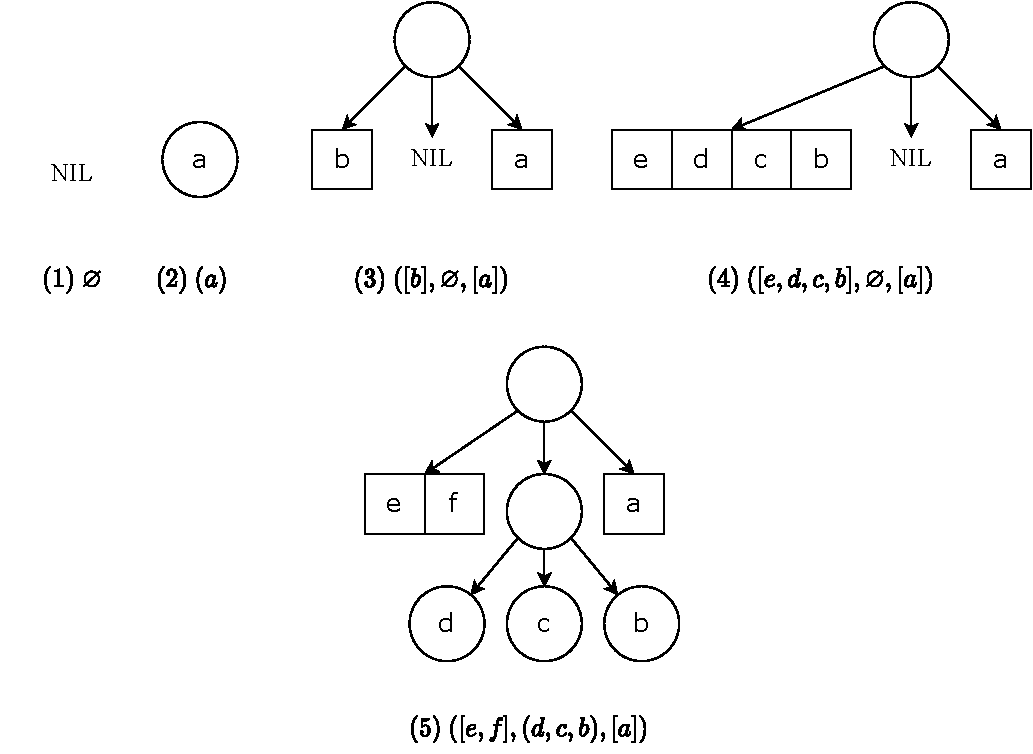
\includegraphics[scale=0.6]{img/ftr-insert}
  \caption{Finger tree example}
  \label{fig:ftr-example}
\end{figure}

As shown in \cref{fig:ftr-example}. (1) is $\nil$, (2) is a singleton, (3) has two element in $f$ and $r$ for each. When add more, $f$ may exceed 2-3 tree, as in (4). We need re-balance as in (5). There are two elements in $f$, the middle is singleton of a 2-3 tree. These examples are list as below:

\btab{ll}
$\nil$ & {\lstinline|Empty|} \\
$(a)$ & {\lstinline|Lf a|} \\
$([b], \nil, [a])$ & {\lstinline|Tr [b] Empty [a]|}\\
$([e, d, c, b], \nil, [a])$ & {\lstinline|Tr [e, d, c, b] Empty [a]|}\\
$([f, e], (d, c, b), [a])$ & {\lstinline|Tr [f, e] Lf (Br3 d c b) [a]|}\\
\etab

\index{Finger tree!insert to left}

In (5), the middle component is a singleton leaf. Finger tree is recursive, apart from $f$ and $r$, the middle is a deeper finger tree of type $Tree\ (Node\ a)$. One more wrap, one level deeper. Summarize above examples, we define insert $a$ to tree $T$ as below:

\begin{enumerate}
\item If $T = \nil$, the result is a singleton $(a)$;
\item If $T = (b)$ is a leaf, the result is $([a], \nil, [b])$;
\item For $T = (f, t, r)$, if there are $\leq 3$ elements in $f$, we insert $a$ to $f$, otherwise ($> 3$), extract the last 3 elements from $f$ to a 2-3 tree $t'$, recursively insert $t'$ to $t$, then insert $a$ to $f$.
\end{enumerate}

\be
\begin{array}{rcl}
insert\ a\ \nil & = & (x) \\
insert\ a\ (b) & = & ([a], \nil, [b]) \\
insert\ a\ ([b, c, d, e], t, r) & = & ([a, b], insert\ (c, d, e)\ t, r) \\
insert\ a\ (f, t, r) & = & (a \cons f, t, r) \\
\end{array}
\ee

The insert performance is constant time except for the recursive case. The recursion time is proportion to the height of the tree $h$. Because of 2-3 trees, it's balanced, hence $h = O(\lg n)$, where $n$ is the number of elements. When distribute the recursion to other cases, the amortized performance is constant time\cite{okasaki-book}\cite{finger-tree-2006}. We can repeatedly insert a list of elements by folding:

\be
xs \gg t = foldr\ insert\ t\ xs
\ee

\begin{Exercise}\label{ex:finger-tree-insert}
\Question{Eliminate recursion, implement insert with loop.}
\end{Exercise}

\begin{Answer}[ref = {ex:finger-tree-insert}]
\Question{Eliminate recursion, implement insert with loop.

Let $\textproc{Mid}(T) = t$ access the middle part of tree $T = (f, t, r)$.

\begin{algorithmic}[1]
\Function{Insert}{$x, T$}
  \State $n = (x)$
  \State $\perp \gets p \gets ([\ ], T, [\ ])$
  \While{$|\textproc{Front}(T)| \geq 3$}
    \State $f \gets \textproc{Front}(T)$
    \State $n \gets (f[2], f[3], ...)$
    \State $\textproc{Front}(T) \gets [n, f[1]]$
    \State $p \gets T$
    \State $T \gets$ \Call{Mid}{$T$}
  \EndWhile
  \If{$T =$ NIL}
    \State $T \gets ([n], \text{NIL}, [\ ])$
  \ElsIf{ $|\textproc{Front}(T)| = 1$ and $\textproc{Rear}(T) = [\ ]$}
    \State \Call{Rear}{$T$} $\gets$ \Call{Front}{$T$}
    \State \Call{Front}{$T$} $\gets [n]$
  \Else
    \State \textproc{Insert}(\Call{Front}{$T$}, $n$)
  \EndIf
  \State \Call{Mid}{$p$} $\gets T$
  \State $T \gets$ \Call{Mid}{$\perp$}, \Call{Mid}{$\perp$} $\gets$ NIL
  \State \Return $T$
\EndFunction
\end{algorithmic}

We wrap $x$ in a leaf $(x)$. If there are more than 3 elements in $f$, we go top-down along the middle part. We extract the elements except the first one in $f$ out, wrap them in a node $n$ (depth + 1), then insert $n$ to the middle. We form $n$ and the remaining in $f$ as the new $f$ finger. At the end of traverse, we either reach an empty tree, or a tree can hold more elements in $f$. For empty tree case, we create a new leaf node; otherwise, we insert $n$ to the head of $f$. We return the root $T$. To simplify implementation, we create a special $\perp$ node as the parent of the root.}
\end{Answer}

\subsection{Extract}
\index{Finger tree!Remove from left}

We implement extract as the reverse of \textit{insert}.

\be
\begin{array}{rcl}
extract\ (a) & = & (a, \nil) \\
extract\ ([a], \nil, [b]) & = & (a, (b)) \\
extract\ ([a], \nil, b \cons bs) & = & (a, ([b], \nil, bs)) \\
extract\ ([a], t, r) & = & (a, (toList\ f, t', r)), \text{where}: (f, t') = extract\ t \\
extract\ (a \cons as, t, r) & = & (a, (as, t, r)) \\
\end{array}
\ee

Where \textit{toList} flatten a 2-3 tree to list:

\be
\begin{array}{rcl}
toList\ (a, b) & = & [a, b] \\
toList\ (a, b, c) & = & [a, b, c] \\
\end{array}
\ee

We skip error handling (e.g., extract from empty tree). If the tree is a singleton leaf, the result is empty; if there are two elements, the result is a singleton; if $f$ is a singleton list, the middle is empty, while $r$ isn't empty, we extract the only one in $f$, then borrow one from $r$ to $f$; if the middle isn't empty, we recursively extract a node from the middle, flatten that node to list to replace $f$ (the original one is extracted). If $f$ has more than one element, we extract the first. \Cref{fig:ftr-uncons-example} gives examples that extract 2 elements.


\begin{figure}[htbp]
  \centering
  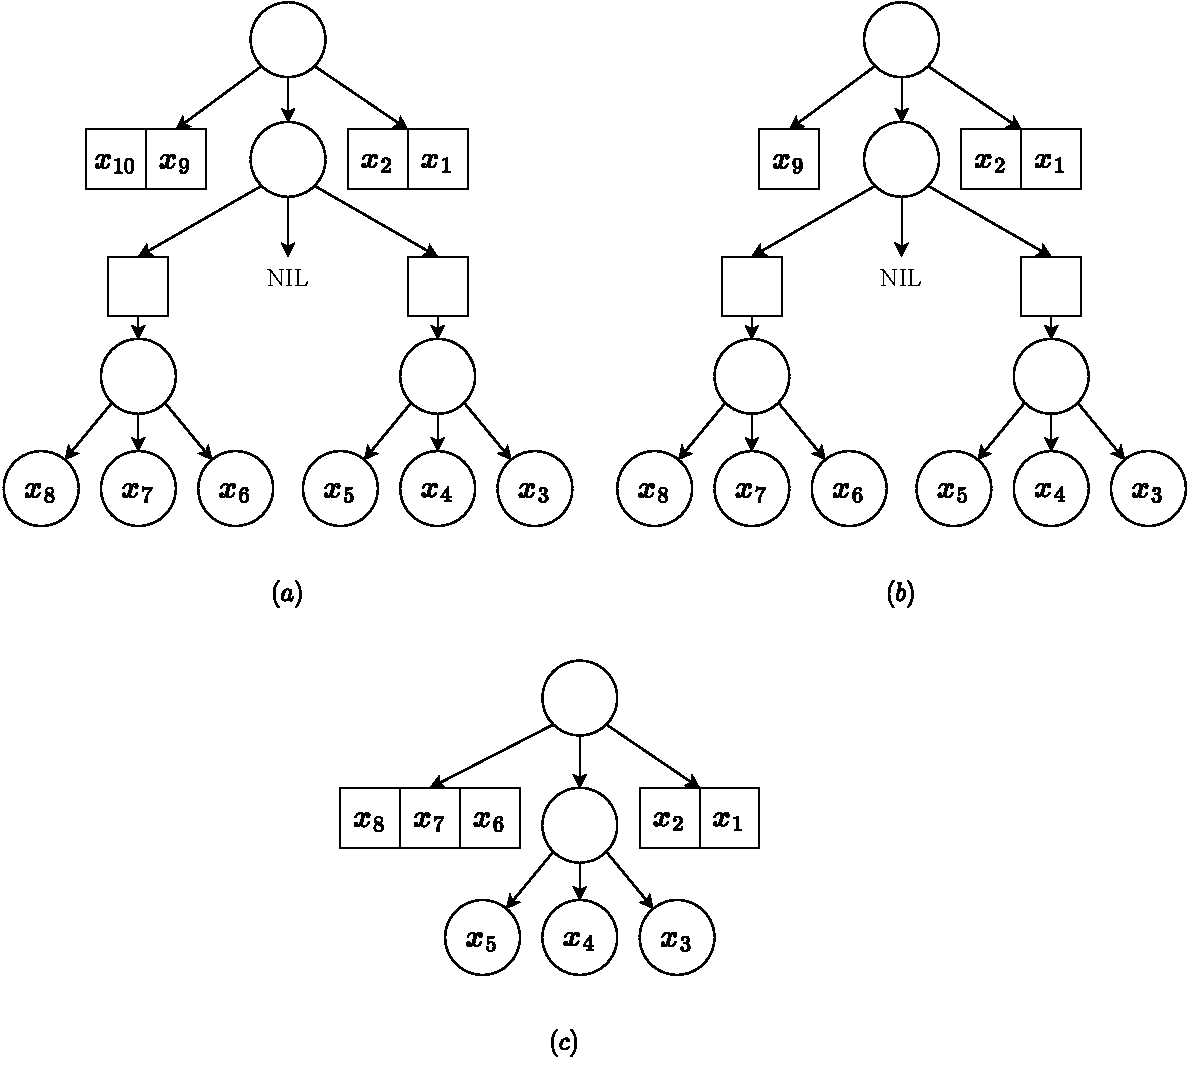
\includegraphics[scale=0.55]{img/ftr-uncons}
  \caption{Extract: (a) A sequence of 10 elements. (b) Extract one, $f$ becomes a singleton list. (c) Extract another, borrow an element from the middle, flatten the 2-3 tree to a list as the new $f$.}
  \label{fig:ftr-uncons-example}
\end{figure}

We can define \textit{head}, \textit{tail} with \textit{extract}.

\be
\begin{cases}
head & = fst \circ extract \\
tail & = snd \circ extract \\
\end{cases}
\ee

\begin{Exercise}\label{ex:finger-tree-del}
\Question{Eliminate recursion, implement extract in loops.}
\end{Exercise}

\begin{Answer}[ref = {ex:finger-tree-del}]
\Question{Eliminate recursion, implement extract in loops.

We borrow node from the middle when $f$ is empty. However, the tree may not well formed, e.g., both $f$ and the middle are empty. It is caused by splitting.

\begin{center}
  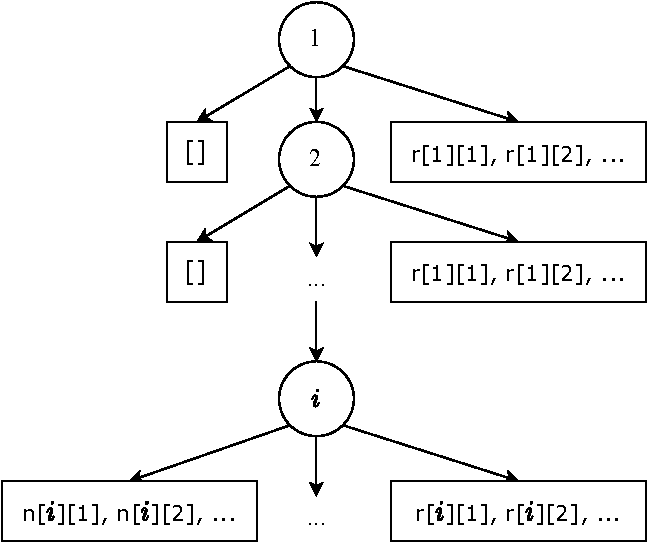
\includegraphics[scale=0.5]{img/ftr-illed-1}
  \captionof{figure}{The $f$ isn't empty at level $i$.}
  \label{fig:ftr-illed-form}
\end{center}

To extract the first element, we need a top-bottom pass, locate a sub-tree, either $f$ isn't empty, or both $f$ and the middle are empty as shown in \cref{fig:ftr-illed-form}. For the former, we extract the first node from $f$; for the latter, we swap $f$ and $r$, convert it to the former case. If the node extracted from $f$ isn't a leaf, we need go on extracting. We back track along the parent, till extract a leaf and reach to the root, as shown in \cref{fig:ftr-illed-extract}.

\begin{center}
  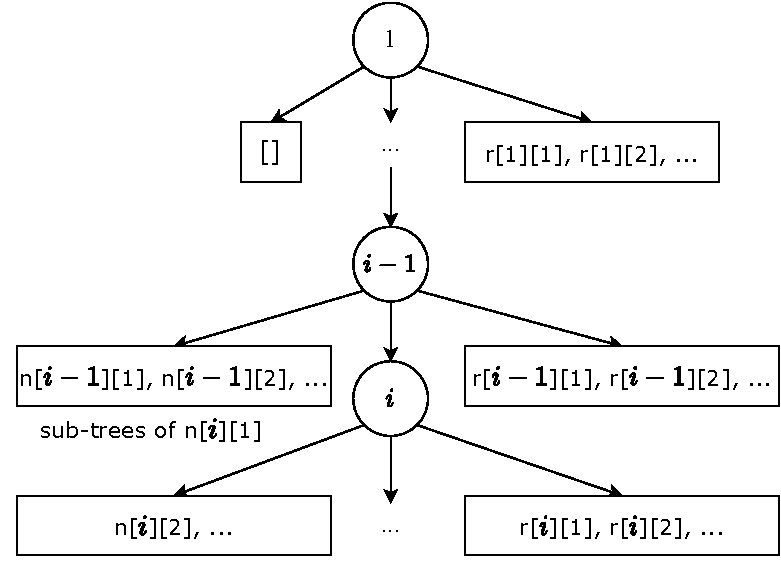
\includegraphics[scale=0.5]{img/ftr-illed-2} \\
  Extract the first $n[i][1]$, move its sub-tree to $f$ in upper level.\\
  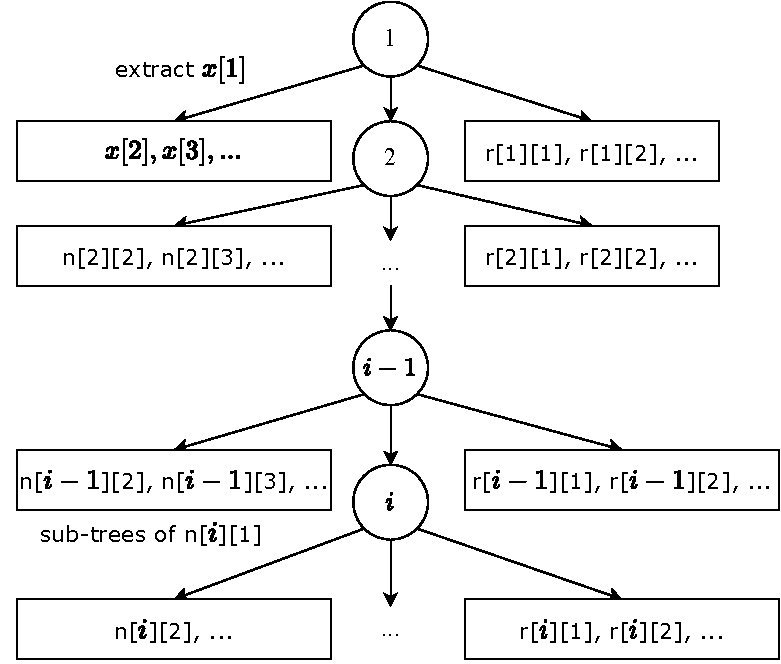
\includegraphics[scale=0.5]{img/ftr-illed-i} \\
  Repeat $i$ times, extract $x[1]$. \\
  \captionof{figure}{Bottom up back track to extract a leaf.}
  \label{fig:ftr-illed-extract}
\end{center}

Assume the tree isn't empty, we implement extract as below:

\begin{algorithmic}[1]
\Function{Extract}{$T$}
  \State $\perp \gets ([], T, [])$
  \While{\Call{Front}{$T$} $= [\ ]$ and \Call{Mid}{$T$} $\neq $ NIL}
    \State $T \gets$ \Call{Mid}{$T$}
  \EndWhile

  \If{\Call{Front}{$T$} $ = [\ ]$ and \Call{Rear}{$T$} $\neq [\ ]$}
    \State \textproc{Exchange} \Call{Front}{$T$} $\leftrightarrow$ \Call{Rear}{$T$}
  \EndIf

  \State $f \gets$ \Call{Front}{$T$}, $r \gets$ \Call{Rear}{$T$}
  \State $n \gets (f[1], f[2], ...)$ \Comment{$n$ is 2-3 tree}
  \Repeat
    \State \Call{Front}{$T$} $\gets [n_2, n_3, ..]$
    \State $n \gets n_1$
    \State $T \gets $ \Call{Parent}{$T$}
    \If{\Call{Mid}{$T$} becomes empty}
      \State \Call{Mid}{$T$} $\gets$ NIL
    \EndIf
  \Until{$n$ is leaf}
  \State \Return (\Call{Elem}{$n$}, \Call{Mid}{$\perp$})
\EndFunction
\end{algorithmic}

Where function \textproc{Elem}($n$) access the element in sub-tree $n$. We need change the way to access the first/last element of finger tree. If the finger is empty, and the middle isn't empty, we need search along the middle.

\begin{algorithmic}[1]
\Function{First-Leaf}{$T$}
  \While{\Call{Front}{$T$} $ = [\ ]$ and \Call{Mid}{$T$} $\neq$ NIL}
    \State $T \gets$ \Call{Mid}{$T$}
  \EndWhile
  \If{\Call{Front}{$T$} $ = [\ ]$ and \Call{Rear}{$T$} $\neq [\ ]$}
    \State $n \gets$ \Call{Rear}{$T$}[1]
  \Else
    \State $n \gets$ \Call{Front}{$T$}[1]
  \EndIf
  \While{$n$ is NOT leaf}
    \State $n \gets n_1$
  \EndWhile
  \State \Return $n$
\EndFunction
\Statex
\Function{First}{$T$}
  \State \Return \textproc{Elem}(\Call{First-Leaf}{$T$})
\EndFunction
\end{algorithmic}

In the second loop, if the node is not a leaf, we need traverse along the first sub-tree. The method to access the last element is symmetric.
}
\end{Answer}

\subsection{Append and remove}
\index{Finger tree!Append to right}

We implement append, remove on right symmetrically.

\be
\begin{array}{rcl}
append\ \nil\ a & = & (a) \\
append\ (a)\ b & = & ([a], \nil, [b]) \\
append\ (f, t, [a, b, c, d])\ e & = & (f, append\ t\ (a, b, c), [d, e]) \\
append\ (f, t, r)\ a & = & (f, t, r \doubleplus [a]) \\
\end{array}
\ee

If there are no more 4 elements in $r$, we append the new element to tail of $r$. Otherwise, we extract the first 3 from $r$, form a new 2-3 tree, and recursively append it to the middle. We can repeatedly append a list of elements by folding from left:

\be
t \ll xs = foldl\ append\ t\ xs
\ee

\index{Finger tree!Remove from right}

The remove is reversed operation of append:

\be
\begin{array}{rcl}
remove\ (a) & = & (\nil, a) \\
remove\ ([a], \nil, [b]) & = & ((a), b) \\
remove\ (f, \nil, [a]) & = & ((init f, \nil, [last f]), a) \\
remove\ (f, t, [a]) & = & ((f, t', toList\ r), a), \text{where}: (t', r) = remove\ t \\
remove\ (f, t, r) & = & ((f, t, init\ r), last\ r) \\
\end{array}
\ee

Where \textit{last} accesses the last element of a list, \textit{init} returns the rest (see chapter 1).

\subsection{concatenate}
\index{Finger tree!Concatenate}

When concatenate two none empty finger trees $T_1 = (f_1, t_1, r_1)$, $T_2 = (f_2, t_2, r_2)$, we use $f_1$ as the result front $f$, $r_2$ as the result rear $r$. Then merge $t_1, r_1, f_2, t_2$ as the middle tree. Because both $r_1$ and $f_2$ are list of nodes, it equivalent to the below problem:

\[
merge\ t_1\ (r_1 \doubleplus f_2)\ t_2 = ?
\]

Both $t_1$ and $t_2$ are finger trees deeper than $T_1$ and $T_2$ a level. If the type of element in $T_1$ is $a$, then the type of element in $t_1$ $Node\ a$. We recursively merge, keep the front of $t_1$ and rear of $t_2$, then further merge the middle of $t_1$, $t_2$, and the rear of $t_1$, the front of $t_2$.

\be
\begin{array}{rcl}
merge\ \nil\ ts\ t_2 & = & ts \gg t_2 \\
merge\ t_1\ ts\ \nil & = & t_1 \ll ts \\
merge\ (a)\ ts\ t_2 & = & merge\ \nil\ (a \cons ts)\ t_2 \\
merge\ t_1\ ts\ (a) & = & merge\ t_1\ (ts \doubleplus [a])\ \nil \\
merge\ (f_1, t_1, r_1)\ ts\ (f_2, t_2, r_2) & = & (f_1, merge\ t_1\ (nodes\ (r_1 \doubleplus ts \doubleplus f_2))\ t_2, r_2) \\
\end{array}
\label{eq:merge-recursion}
\ee

Where $nodes$ collects elements to a list of 2-3 trees. This is because type of the element in the middle is deeper than the finger.

\be
\begin{array}{rcl}
nodes\ [a, b] & = & [(a, b)] \\
nodes\ [a, b, c] & = & [(a, b, c)] \\
nodes\ [a, b, c, d] & = & [(a, b), (c, d)] \\
nodes\ (a \cons b \cons c \cons ts) & = & (a, b, c) \cons nodes\ ts \\
\end{array}
\ee

We then define finger tree concatenation with $merge$:

\be
(f_1, t_1, r_1) \doubleplus (f_2, t_2, r_2) = (f_1, merge\ t_1\ (r_1 \doubleplus f_2)\ t_2, r_2)
\ee

Compare with \cref{eq:merge-recursion}, concatenation is essentially merge, we can define them in a unified way:

\be
T_1 \doubleplus T_2 = merge\ T_1\ [\ ]\ T_2
\ee

The performance is proportion to the number of recursions, which is the smaller height of the two trees. The 2-3 trees are balanced, the height is $O(\lg n)$, where $n$ is the number of elements. In edge cases, merge performs as same as insert (call \textit{insert} at most 8 times) in amortized constant time; In worst case, the performance is $O(m)$, where $m$ is the height difference between the two trees. The overall performance is bound $O(\lg n)$, where $n$ is the total elements of the two trees.

\subsection{Random access}
\index{Finger tree!Random access}

The idea is to turn random access into tree search. To avoid repeatedly compute tree size, we augment a size variable $s$ to each branch node as $(s, f, t, r)$.

\begin{Haskell}
data Tree a = Empty
            | Lf a
            | Tr Int [a] (Tree (Node a)) [a]
\end{Haskell}

\be
\begin{array}{rcl}
size\ \nil & = & 0 \\
size\ (x) & = & size\ x \\
size\ (s, f, t, r) & = & s \\
\end{array}
\ee

Here $size\ (x)$ is not necessarily 1. $x$ can be a deeper node, like $Node\ a$. It is only 1 at level one. For termination, we wrap $x$ as an element cell $(x)_e$, and define $size\ (x)_e = 1$ (see the example in appendix).

\be
\begin{cases}
x \lhd t = insert\ (x)_e\ t \\
t \rhd x = append\ t\ (x)_e \\
\end{cases}
\ee

and:

\be
\begin{cases}
xs \ll t = foldr\ (\lhd)\ t\ xs \\
t \gg xs = foldl\ (\rhd)\ t\ xs \\
\end{cases}
\ee

We also need calculate the size of a 2-3 tree:

\be
\begin{array}{rcl}
size\ (t_1, t_2) & = & size\ t_1 + size\ t_2 \\
size\ (t_1, t_2, t_3) & = & size\ t_1 + size\ t_2 + size\ t_3 \\
\end{array}
\ee

Given a list of nodes (e.g., finger at deeper level), we calculate size from $sum \circ (map\ size)$. We need update the size when insert or delete element. With size augmented, we can lookup the tree for any position $i$. The finger tree $(s, f, t, r)$ has recursive structure. Let the size of these components be $s_f, s_t, s_r$, and $s = s_f + s_t + s_r$. If $i \leq s_f$, the location is in $f$, we further lookup $f$; if $s_f < i \leq s_f + s_t$, then the location is in $t$, we need recursively lookup $t$; otherwise, we lookup $r$. We also need handle leaf case of $(x)$. We use a pair $(i, t)$ to define the position $i$ at data structure $t$, and define $lookup_T$ as below:

\be
\begin{array}{rcl}
lookup_T\ i\ (x) & = & (i, x) \\
lookup_T\ i\ (s, f, t, r) & = & \begin{cases}
  i < s_f: & lookup_s\ i\ f \\
  s_f \leq i < s_f + s_t: & lookup_N\ (lookup_T\ (i - s_f)\ t) \\
  \text{otherwise}: & lookup_s\ (i - s_f - s_t)\ r \\
\end{cases}
\end{array}
\ee

Where $s_f = sum\ (map\ size\ f), s_t = size\ t$, are the sizes of the first two components. When lookup location $i$, if the tree is a leaf $(x)$, the result is $(i, x)$; otherwise we need figure out which component among $(s, f, t, r)$ that $i$ points to. If it either in $f$ or $r$, then we lookup the figure:

\be
\begin{array}{rcl}
lookup_s\ i\ (x \cons xs) = \begin{cases}
  i < size\ x: & (i, x) \\
  \text{otherwise}: & lookup_s\ (i - size\ x)\ xs \\
\end{cases}
\end{array}
\ee

If $i$ is in some element $x$ ($i < size\ x$), we return $(i, x)$; otherwise, we continue looking up the rest elements. If $i$ points to the middle $t$, we recursively lookup to obtain a place $(i', m)$, where $m$ is a 2-3 tree. We next lookup $m$:

\be
\begin{array}{rcl}
lookup_N\ i\ (t_1, t_2) & = & \begin{cases}
  i < size\ t_1: & (i, t_1) \\
  \text{otherwise}: & (i - size\ t_1, t_2) \\
\end{cases} \\
lookup_N\ i\ (t_1, t_2, t_3) & = & \begin{cases}
  i < size\ t_1: & (i, t_1) \\
  size\ t_1 \leq i < size\ t_1 + size\ t_2: & (i - size\ t_1, t_2) \\
  \text{otherwise}: & (i - size\ t_1 - size\ t_2, t_3) \\
\end{cases} \\
\end{array}
\ee

Because we previously wrapped $x$ inside $(x)_e$, we need extract $x$ out finally:

\be
T[i] = \begin{cases}
  \text{if}\ lookup_T\ i\ T = (i', (x)_e): & \textit{Just}\ x \\
  \text{otherwise}: & \textit{Nothing}
\end{cases}
\ee

We return the result of type $\textit{Maybe}\ a = \textit{Nothing} | \textit{Just}\ a$, means either found, or lookup failed\footnote{Many programming environments provide equivalent tool, like the \texttt{Optional<T>} in Java/C++.}. The random access looks up the finger tree recursively, proportion to the tree depth. Because finger tree is balanced, the performs is bound to $O(\lg n)$, where $n$ is the number of elements.

\index{MTF}
We achieved balanced performance with finger tree implementation. The operations at head and tail are bound to amortized constant time, concatenation, split, and random access are in logarithm time\cite{hackage-ftr}. By the end of this chapter, we've seen many elementary data structures. They are useful to solve some classic problems. For example, we can use sequence to implement MTF (move-to-front\footnote{Used in Burrows-Wheeler transform (BWT) data compression algorithm.}) encoding algorithm\cite{mtf-wiki}. MTF move any element at position $i$ to the front of the sequence:

\[
mtf\ i\ S = x \lhd S', \text{where}(x, S') = \textit{extractAt}\ i\ S
\]

In the next chapters, we'll go through the classic divide and conquer sorting algorithms, including quick sort, merge sort and their variants; then give the string matching algorithms and elementary search algorithms.

\begin{Exercise}\label{ex:finger-tree-index}
\Question{For random access, how to handle empty tree $\nil$ and out of bound cases?}
\Question{Implement $cut\ i\ S$, split sequence $S$ at position $i$.}
\end{Exercise}

\begin{Answer}[ref = {ex:finger-tree-index}]
\Question{For random access, how to handle empty tree $\nil$ and out of bound cases?

We check boundaries during random access, for example:
\[
\begin{array}{rcl}
\nil [i] & = & \textit{Nothing} \\
T [i] & = & \begin{cases}
  i < 0\ \text{or}\ i \geq size\ T: & \textit{Nothing} \\
  \text{otherwise}: & ...
\end{cases}
\end{array}
\]
}
\Question{Implement $cut\ i\ S$, split sequence $S$ at position $i$.

We give an implementation based on the tree definition in appendix. We first do boundary check, if $0 \leq i < size\ s$, we next call \textit{catTree\ i\ S} to split the tree:

\begin{Haskell}
cut :: Int -> Seq a -> (Seq a, Maybe a, Seq a)
cut i (Seq xs) | i < 0 = (Seq Empty, Nothing, Seq xs)
               | i < size xs = case cutTree i xs of
                 (a, Just (Place _ (Elem x)), b) -> (Seq a, Just x, Seq b)
                 (a, Nothing, b) -> (Seq a, Nothing, Seq b)
               | otherwise = (Seq xs, Nothing, Seq Empty)
\end{Haskell}

\textit{cutTree} splits the tree in three parts: left, middle, and right. We wrap the middle in \textit{Maybe} type to handle the not found case; when found, the result is a pair of position $i'$ and node $a$, wrapped in the type of \textit{Place}. if $i$ points to finger $f$ or $r$, we call \textit{cutList} to further split, then build the result; if $i$ points to middle, we recursively cut the middle to obtain a place $\textit{Place}\ i'\ a$, then cut the 2-3 tree $a$ at position $i'$:

\begin{Haskell}
cutTree :: (Sized a) => Int -> Tree a -> (Tree a, Maybe (Place a), Tree a)
cutTree _ Empty = (Empty, Nothing, Empty)
cutTree i (Lf a) | i < size a = (Empty, Just (Place i a), Empty)
                 | otherwise = (Lf a, Nothing, Empty)
cutTree i (Br s f m r)
  | i < sf = case cutList i f of
               (xs, x, ys) -> (Empty <<< xs, x, tree ys m r)
  | i < sm = case cutTree (i - sf) m of
               (t1, Just (Place i' a), t2) -> let (xs, x, ys) = cutNode i' a
                 in (tree f t1 xs, x, tree ys t2 r)
  | i < s  = case cutList (i - sm) r of
               (xs, x, ys) -> (tree f m xs, x, ys >>> Empty)
  where
    sf = sum $ map size f
    sm = sf + size m
\end{Haskell}

Where $tree\ f\ m\ r$ builds a finger tree, and simplify the result:

\begin{Haskell}
tree as Empty [] = as >>> Empty
tree [] Empty bs = Empty <<< bs
tree [] m r = Br (size m + sum (map size r)) (nodesOf f) m' r
    where (f, m') = uncons m
tree f m [] = Br (size m + sum (map size f)) f m' (nodesOf r)
    where (m', r) = unsnoc m
tree f m r = Br (size m + sum (map size f) + sum (map size r)) f m r
\end{Haskell}

We implement the finger cut and 2-3 tree cut as below:

\begin{Haskell}
cutList :: (Sized a) => Int -> [a] -> ([a], Maybe (Place a), [a])
cutList _ [] = ([], Nothing, [])
cutList i (x:xs) | i < sx = ([], Just (Place i x), xs)
                 | otherwise = let (xs', y, ys) = cutList (i - sx) xs
                               in (x:xs', y, ys)
  where sx = size x

cutNode :: (Sized a) => Int -> Node a -> ([a], Maybe (Place a), [a])
cutNode i (Tr2 _ a b) | i < sa = ([], Just (Place i a), [b])
                      | otherwise = ([a], Just (Place (i - sa) b), [])
  where sa = size a
cutNode i (Tr3 _ a b c) | i < sa = ([], Just (Place i a), [b, c])
                        | i < sab = ([a], Just (Place (i - sa) b), [c])
                        | otherwise = ([a, b], Just (Place (i - sab) c), [])
  where sa = size a
        sab = sa + size b
\end{Haskell}

With \textit{cut} defined, we can update or delete any element at given position, move to front (MTF), they all bound to $O(\lg n)$ time.

\begin{Haskell}
setAt s i x = case cut i s of
  (_, Nothing, _) -> s
  (xs, Just y, ys) -> xs +++ (x <| ys)

extractAt s i = case cut i s of (xs, Just y, ys) -> (y, xs +++ ys)

moveToFront i s = if i < 0 || i >= size s then s
                  else let (a, s') = extractAt s i in a <| s'
\end{Haskell}
}
\end{Answer}

\section{Appendix - example programs}

Binary random access list (forest):

\lstset{frame = single}
\begin{Haskell}
data Tree a = Leaf a
            | Node Int (Tree a) (Tree a)

type BRAList a = [Tree a]

size (Leaf _) = 1
size (Node sz _ _) = sz

link t1 t2 = Node (size t1 + size t2) t1 t2

insert x = insertTree (Leaf x) where
    insertTree t [] = [t]
    insertTree t (t':ts) = if size t < size t' then  t:t':ts
                           else insertTree (link t t') ts

extract ((Leaf x):ts) = (x, ts)
extract ((Node _ t1 t2):ts) = extract (t1:t2:ts)

head' = fst . extract
tail' = snd . extract

getAt i (t:ts) | i < size t = lookupTree i t
               | otherwise = getAt (i - size t) ts
  where
    lookupTree 0 (Leaf x) = x
    lookupTree i (Node sz t1 t2)
        | i < sz `div` 2 = lookupTree i t1
        | otherwise = lookupTree (i - sz `div` 2) t2
\end{Haskell}

Numeric representation of binary random access list:

\begin{Haskell}
data Digit a = Zero | One (Tree a)

type RAList a = [Digit a]

insert x = add (Leaf x) where
  add t [] = [One t]
  add t (Zero:ts) = One t : ts
  add t (One t' :ts) = Zero : add (link t t') ts

minus [One t] = (t, [])
minus (One t:ts) = (t, Zero:ts)
minus (Zero:ts) = (t1, One t2:ts') where
    (Node _ t1 t2, ts') = minus ts

head' ts = x where (Leaf x, _) = minus ts
tail' = snd . minus
\end{Haskell}

Paired-array sequence:

\begin{lstlisting}[language = Bourbaki]
Data Seq<K> {
    [K] front = [], rear = []
}

Int length(S<K> s) = length(s.front) + length(s.rear)

void insert(K x, Seq<K> s) = append(x, s.front)

void append(K x, Seq<K> s) = append(x, s.rear)

K get(Int i, Seq<K> s) {
    Int n = length(s.front)
    return if i < n then s.front[n - i - 1] else s.rear[i - n]
}
\end{lstlisting}

Concatenate-able list:

\begin{Haskell}
data CList a = Empty | CList a (Queue (CList a))

wrap x = CList x emptyQ

x ++ Empty = x
Empty ++ y = y
(CList x q) ++ y = CList x (push q y)

fold f z q | isEmpty q = z
           | otherwise = (top q) `f` fold f z (pop q)

concat = fold (++) Empty

insert x xs = (wrap x) ++ xs
append xs x = xs ++ wrap x

head (CList x _) = x
tail (CList _ q) = concat q
\end{Haskell}

Finger tree:

\begin{Haskell}
-- 2-3 tree
data Node a = Tr2 Int a a
            | Tr3 Int a a a

-- finger tree
data Tree a = Empty
            | Lf a
            | Br Int [a] (Tree (Node a)) [a] -- size, front, mid, rear

newtype Elem a = Elem { getElem :: a } -- wrap element

newtype Seq a = Seq (Tree (Elem a)) -- sequence

class Sized a where  -- support size measurement
  size :: a -> Int

instance Sized (Elem a) where
  size _ = 1  -- 1 for any element

instance Sized (Node a) where
  size (Tr2 s _ _) = s
  size (Tr3 s _ _ _) = s

instance Sized a => Sized (Tree a) where
  size Empty = 0
  size (Lf a) = size a
  size (Br s _ _ _) = s

instance Sized (Seq a) where
  size (Seq xs) = size xs

tr2 a b = Tr2 (size a + size b) a b
tr3 a b c = Tr3 (size a + size b + size c) a b c

nodesOf (Tr2 _ a b) = [a, b]
nodesOf (Tr3 _ a b c) = [a, b, c]

-- left
x <| Seq xs = Seq (Elem x `cons` xs)

cons :: (Sized a) => a -> Tree a -> Tree a
cons a Empty = Lf a
cons a (Lf b) = Br (size a + size b) [a] Empty [b]
cons a (Br s [b, c, d, e] m r) = Br (s + size a) [a, b] ((tr3 c d e) `cons` m) r
cons a (Br s f m r) = Br (s + size a) (a:f) m r

head' (Seq xs) = getElem $ fst $ uncons xs
tail' (Seq xs) = Seq $ snd $ uncons xs

uncons :: (Sized a) => Tree a -> (a, Tree a)
uncons (Lf a) = (a, Empty)
uncons (Br _ [a] Empty [b]) = (a, Lf b)
uncons (Br s [a] Empty (r:rs)) = (a, Br (s - size a) [r] Empty rs)
uncons (Br s [a] m r) = (a, Br (s - size a) (nodesOf f) m' r)
    where (f, m') = uncons m
uncons (Br s (a:f) m r) = (a, Br (s - size a) f m r)

-- right
Seq xs |> x  = Seq (xs `snoc` Elem x)

snoc :: (Sized a) => Tree a -> a -> Tree a
snoc Empty a = Lf a
snoc (Lf a) b = Br (size a + size b) [a] Empty [b]
snoc (Br s f m [a, b, c, d]) e = Br (s + size e) f (m `snoc` (tr3 a b c)) [d, e]
snoc (Br s f m r) a = Br (s + size a) f m (r ++ [a])

last' (Seq xs) = getElem $ snd $ unsnoc xs
init' (Seq xs) = Seq $ fst $ unsnoc xs

unsnoc :: (Sized a) => Tree a -> (Tree a, a)
unsnoc (Lf a) = (Empty, a)
unsnoc (Br _ [a] Empty [b]) = (Lf a, b)
unsnoc (Br s f@(_:_:_) Empty [a]) = (Br (s - size a) (init f) Empty [last f], a)
unsnoc (Br s f m [a]) = (Br (s - size a) f m' (nodesOf r), a)
    where (m', r) = unsnoc m
unsnoc (Br s f m r) = (Br (s - size a) f m (init r), a) where a = last r

-- concatenate
Seq xs +++ Seq ys = Seq (xs >+< ys)

xs >+< ys = merge xs [] ys

t <<< xs = foldl snoc t xs
xs >>> t = foldr cons t xs

merge :: (Sized a) => Tree a -> [a] -> Tree a -> Tree a
merge Empty es t2 = es >>> t2
merge t1 es Empty = t1 <<< es
merge (Lf a) es t2 = merge Empty (a:es) t2
merge t1 es (Lf a) = merge t1 (es++[a]) Empty
merge (Br s1 f1 m1 r1) es (Br s2 f2 m2 r2) =
    Br (s1 + s2 + (sum $ map size es)) f1 (merge m1 (trees (r1 ++ es ++ f2)) m2) r2

trees [a, b] = [tr2 a b]
trees [a, b, c] = [tr3 a b c]
trees [a, b, c, d] = [tr2 a b, tr2 c d]
trees (a:b:c:es) = (tr3 a b c):trees es

-- index
data Place a = Place Int a

getAt :: Seq a -> Int -> Maybe a
getAt (Seq xs) i | i < size xs = case lookupTree i xs of
                     Place _ (Elem x) -> Just x
                 | otherwise = Nothing

lookupTree :: (Sized a) => Int -> Tree a -> Place a
lookupTree n (Lf a) = Place n a
lookupTree n (Br s f m r) | n < sf = lookups n f
                          | n < sm = case lookupTree (n - sf) m of
                                            Place n' xs -> lookupNode n' xs
                          | n < s = lookups (n - sm) r
  where sf = sum $ map size f
        sm = sf + size m

lookupNode :: (Sized a) => Int -> Node a -> Place a
lookupNode n (Tr2 _ a b) | n < sa = Place n a
                         | otherwise = Place (n - sa) b
  where sa = size a
lookupNode n (Tr3 _ a b c) | n < sa = Place n a
                           | n < sab = Place (n - sa) b
                           | otherwise = Place (n - sab) c
  where sa = size a
        sab = sa + size b

lookups :: (Sized a) => Int -> [a] -> Place a
lookups n (x:xs) = if n < sx then Place n x
                   else lookups (n - sx) xs
  where sx = size x
\end{Haskell}

\ifx\wholebook\relax \else
\section{Answers}
\shipoutAnswer

\begin{thebibliography}{99}

\bibitem{okasaki-book}
Chris Okasaki. ``Purely Functional Data Structures''. Cambridge university press, (July 1, 1999), ISBN-13: 978-0521663502

\bibitem{okasaki-ralist}
Chris Okasaki. ``Purely Functional Random-Access Lists''. Functional Programming Languages and Computer Architecture, June 1995, pages 86-95.

\bibitem{CLRS}
Thomas H. Cormen, Charles E. Leiserson, Ronald L. Rivest and Clifford Stein. ``Introduction to Algorithms, Second Edition''. The MIT Press, 2001. ISBN: 0262032937.

\bibitem{learn-haskell}
Miran Lipovaca. ``Learn You a Haskell for Great Good! A Beginner's Guide''. No Starch Press; 1 edition April 2011, 400 pp. ISBN: 978-1-59327-283-8

\bibitem{finger-tree-2006}
Ralf Hinze and Ross Paterson. ``Finger Trees: A Simple General-purpose Data Structure,'' in Journal of Functional Programming 16:2 (2006), pages 197-217. \url{http://www.soi.city.ac.uk/~ross/papers/FingerTree.html}

\bibitem{finger-tree-1977}
Guibas, L. J., McCreight, E. M., Plass, M. F., Roberts, J. R. (1977), "A new representation for linear lists". Conference Record of the Ninth Annual ACM Symposium on Theory of Computing, pp. 49-60.

\bibitem{hackage-ftr}
Generic finger-tree structure. \url{http://hackage.haskell.org/packages/archive/fingertree/0.0/doc/html/Data-FingerTree.html}

\bibitem{mtf-wiki}
Wikipedia. Move-to-front transform. \url{https://en.wikipedia.org/wiki/Move-to-front_transform}

\end{thebibliography}

\expandafter\enddocument
\fi
